\documentclass[10pt,a5paper,twoside]{book}
\usepackage[utf8]{inputenc}
\usepackage[czech]{babel}
\usepackage[T1]{fontenc}
\usepackage{amsmath}
\usepackage{amsfonts}
\usepackage{amssymb}
\usepackage{hyperref}
\usepackage[dvips]{graphicx}
\usepackage[top=2cm, left=1.5cm, bottom=1.5cm, includefoot]{geometry}
\usepackage{eso-pic}
\usepackage{pdfpages}
\usepackage{textpos}
\usepackage{titlesec}
\usepackage{verbatim}
\fontencoding{T1}
\fontfamily{cmss}
\fontseries{m}
\fontshape{n}
\setlength{\belowcaptionskip}{-15pt} % mezera za popiskem obrázku
\usepackage{xcolor}
\usepackage{pdfpages}
\titleformat{\section}
{\color{blue}\normalfont\Large\bfseries}
{\color{blue}\thesection}{1.2em}{}

\newcommand{\autor}[1]{
	\begin{flushright}
	\textit{#1}
	\end{flushright}
}

\newcommand{\nadpis}[2]{
\section*{#1}
	\begin{flushright}
	\textit{#2}
	\end{flushright}
}

\newcommand{\podpis}[1]{
	\begin{flushright}
	\textit{#1}
	\end{flushright}
}

\begin{document} 

\section*{K obrázku na titulní straně}
Obrázek s názvem "Einstein", který je na obálce tohoto jihočasu, nakreslil náš člen Vladan Špaček.\vfill
\section*{Členské příspěvky}
Členské příspěvky na rok 2018 je nutné zaplatit do 14. listopadu. Příspěvky prosím posílejte jako vždy na náš transparentní účet: 2900452466/2010. Platba v hotovosti není možná. Do zprávy pro příjemce uveďte své jméno a příjmení. Studenti a důchodci platí 450 Kč, ostatní 600 Kč.

\section*{Výroční schůze jihočeské pobočky ČAS}
Dne 25. 11. 2017 se na Hvězdárně prof. Františka Nušla v Jindřichově Hradci bude konat výroční schůze Jihočeské pobočky. Začátek schůze je naplánován na 19. hodinu. Bude to jedno z posledních setkaní, které se na této hvězdárně uskuteční před její rekonstrukcí.

\section*{JihoČAS}
Vydává: Jihočeská pobočka České astronomické společnosti.\\
Redakce a adresa pro zasílání příspěvků: Martin Kákona, U Jatek 19/III, 392 01 Soběslav, e-mail: \href{mailto:martin.kakona@astro.cz}{martin.kakona@astro.cz}.\\
Sazba: Roman Dvořák, e-mail: \href{mailto:roman-dvorak@email.cz}{roman-dvorak@email.cz}.\newpage

\nadpis{Noční Astrovlak a Hvězdárna F. Nušla\\aneb\\pára a hvězdy - dvojí fyzika v České kanadě}{Hvězdárna F. Nušla. Jindřichův Hradec\\Jana jirků}


11. srpna, tedy před několika dny, pořádaly Jindřichohradecké místní dráhy a.s. spolu s naší Hvězdárnou akci „Noční Astrovlak“ na úzkorozchodné trase Jindřichův Hradec – Nová Bystřice, za účelem pozorování Perseid i dalších objektů oblohy v dobré tmě. Celé to spočívalo v tom, že kolem půl deváté večer z jindřichohradeckého úzkorozchodného nádraží vyjel vlak tažený parní lokomotivou U 37.002, zvanou „Sedmatřicítka“ která zanedlouho oslaví 120. narozeniny (1898). Zde si lidé mohli prohlédnout frkající, pískající a kouřící historickou parní lokomotivu, vyfotit, natočit. Cílem pak byla obec Hůrky v České kanadě (kousek odtud, dá se říci, že co byste kamenem dohodili, je hraniční přechod do Rakouska v Nové Bystřici).


Jeli jsme v sestavě: Jana Kolářová, Vláďa „Ježíš“ Štefl a moje maličkost vlakem; naším úkolem bylo vlak procházet a rozmlouvat s účastníky, představit jim celou akci, jak bude probíhat, odpovídat na jejich dotazy a poradit jim s kvízem, který jsme na cestu pro ně připravili a podobně. Honza Štrobl, Pavel Kubas a Tomáš Záruba přijeli rovnou do Hůrek dvěma auty s veškerou technikou, kterou mezitím připravili a ustavili.

Počasí přes den nebylo vůbec dobré, honily se bouřky, mraky, pršelo a jak se večer blížil, beznaděj houstla, a to i proto, že ani předpověď na večer nebyla nic moc. Ale po nějaké aktualizaci na stránkách CHMI se ukázalo, že by pozorování přece jen mohlo vyjít. Do Hůrek vlak dorazil cca ve 22:15 a cestou se téměř vyčasilo. Zde jsme měli připravené celkem tři dalekohledy: dva refraktory – Celestron 100/500 mm, Ježíšův Bresser 60/800 mm a jeden Newton, 160/1200 mm. Pro pozorování vyla vyhrazena loučka s dobrým výhledem na východ a velkou část jihu. Západ bohužel na místě cloní vzrostlé stromy a lesy, takže Jupiter ani Saturn jsme neviděli. Zato přelétlo mnoho Perseid, pozorovali jsme některé planetární mlhoviny – M 27, M 57, hvězdokupy M 13 a M 3, dvojhvězdy gama Delfína a Albireo, galaxii v Andromedě atd. Bylo by toho vidět jistě mnohem víc, protože v Hůrkách je opravdu tma, ale obloha nebyla úplně čistá a krátce před půl jedenáctou vyšel Měsíc, čtyři dny po úplňku, tedy ještě v dosti velké fázi. Vyšel skoro přesně na východě, nad rybníkem v lehkých mracích, což vytvořilo úchvatnou scenérii, takže slavil největší úspěch. Přes stále se táhnoucí lehkou „vatu“ po obloze (vůbec si ale nestěžujeme, počasí přes den bylo tak nechutné, že to všechno mohlo dopadnout úplně jinak) vypadal krásně, takže jsme použili na všechny objekty i Měsíc zvětšení od 25x do 240x, to velké když se náš kulatý soused vyšplhal už výš na oblohu a vylezl z mraků.


Pro případ, že by obloha zůstala uražená a dále s námi nemluvila, jsme měli připravenou „mokrou variantu“. Co jiného, než projekci oblohy na plátně, povídání o dalekohledech a optice a další debaty o všem, co koho zajímá v nádražní stodole, zrekonstruované do podoby hospůdky a velkých stanech na loučce poblíž. Naštěstí jsme ji ale nemuseli použít.


Pozorování bylo obohacené také o občerstvení, sestávající se z nápojů a výborných grilovaných klobás. Skončilo pár minut po půlnoci, kdy se Astrovlak s účastníky, tentokrát už bez nás, vydal na cestu zpět do Jindřichova Hradce a my se jali balit, rozebírat, uklízet, nakládat a odjet domů.


Jediné, co mi tak trochu vadilo, bylo to, že JHMD udělaly na svém webu a plakátku několik chyb, ale hlavně to, že s námi nekonzultovaly termín akce a stanovily rovnou pátek a my museli zavřít běžné páteční návštěvní hodiny; pátky se nám nehodí a tím spíš v sezóně a o prázdninách, kdy chodí mnoho návštěvníků na Hvězdárnu na prohlídku oblohy. Ale podařilo se dobře zpropagovat náhradní termín, hned další večer, v sobotu 12. srpna. To také proběhlo kolem 22. hodiny maximum roje Perseid, takže naše Hvězdárna doslova „praskala ve švech“.


Jsem ale přesto nesmírně ráda, že se akce Noční Astrovlak povedla doslova nadprůměrně, sice očekávané počasí zapříčinilo o trochu nižší účast, než byl původní odhad, ale zúčastněných bylo kolem 80 a pár jich přijelo rovnou na místo navíc, bez cesty vlakem. Lidé byli nadšení, spokojení a chválili, což pochopitelně pro nás mnoho znamená.


Ze strany Úzkokolejek jsem se dozvěděla od jejich pracovníka a svého spoluorganizátora, že vedení JHMD bylo více než spokojené s průběhem akce, takže rozhodně stojí o další spolupráci s námi na podobných aktivitách.


Bohužel, hned druhý den po Astrovlaku, 12. srpna, musela U 37.002 nahradit U 47.001 – o polovinu mladší rumunská Resita z roku 1958. Historickou lokomotivu vyřadila z provozu technická závada, takže je nyní v opravě. Prosím, držte s námi palce Sedmatřicítce, ať se povede znovu ji vrátit na trať!

\begin{figure}[ht!]
\centering
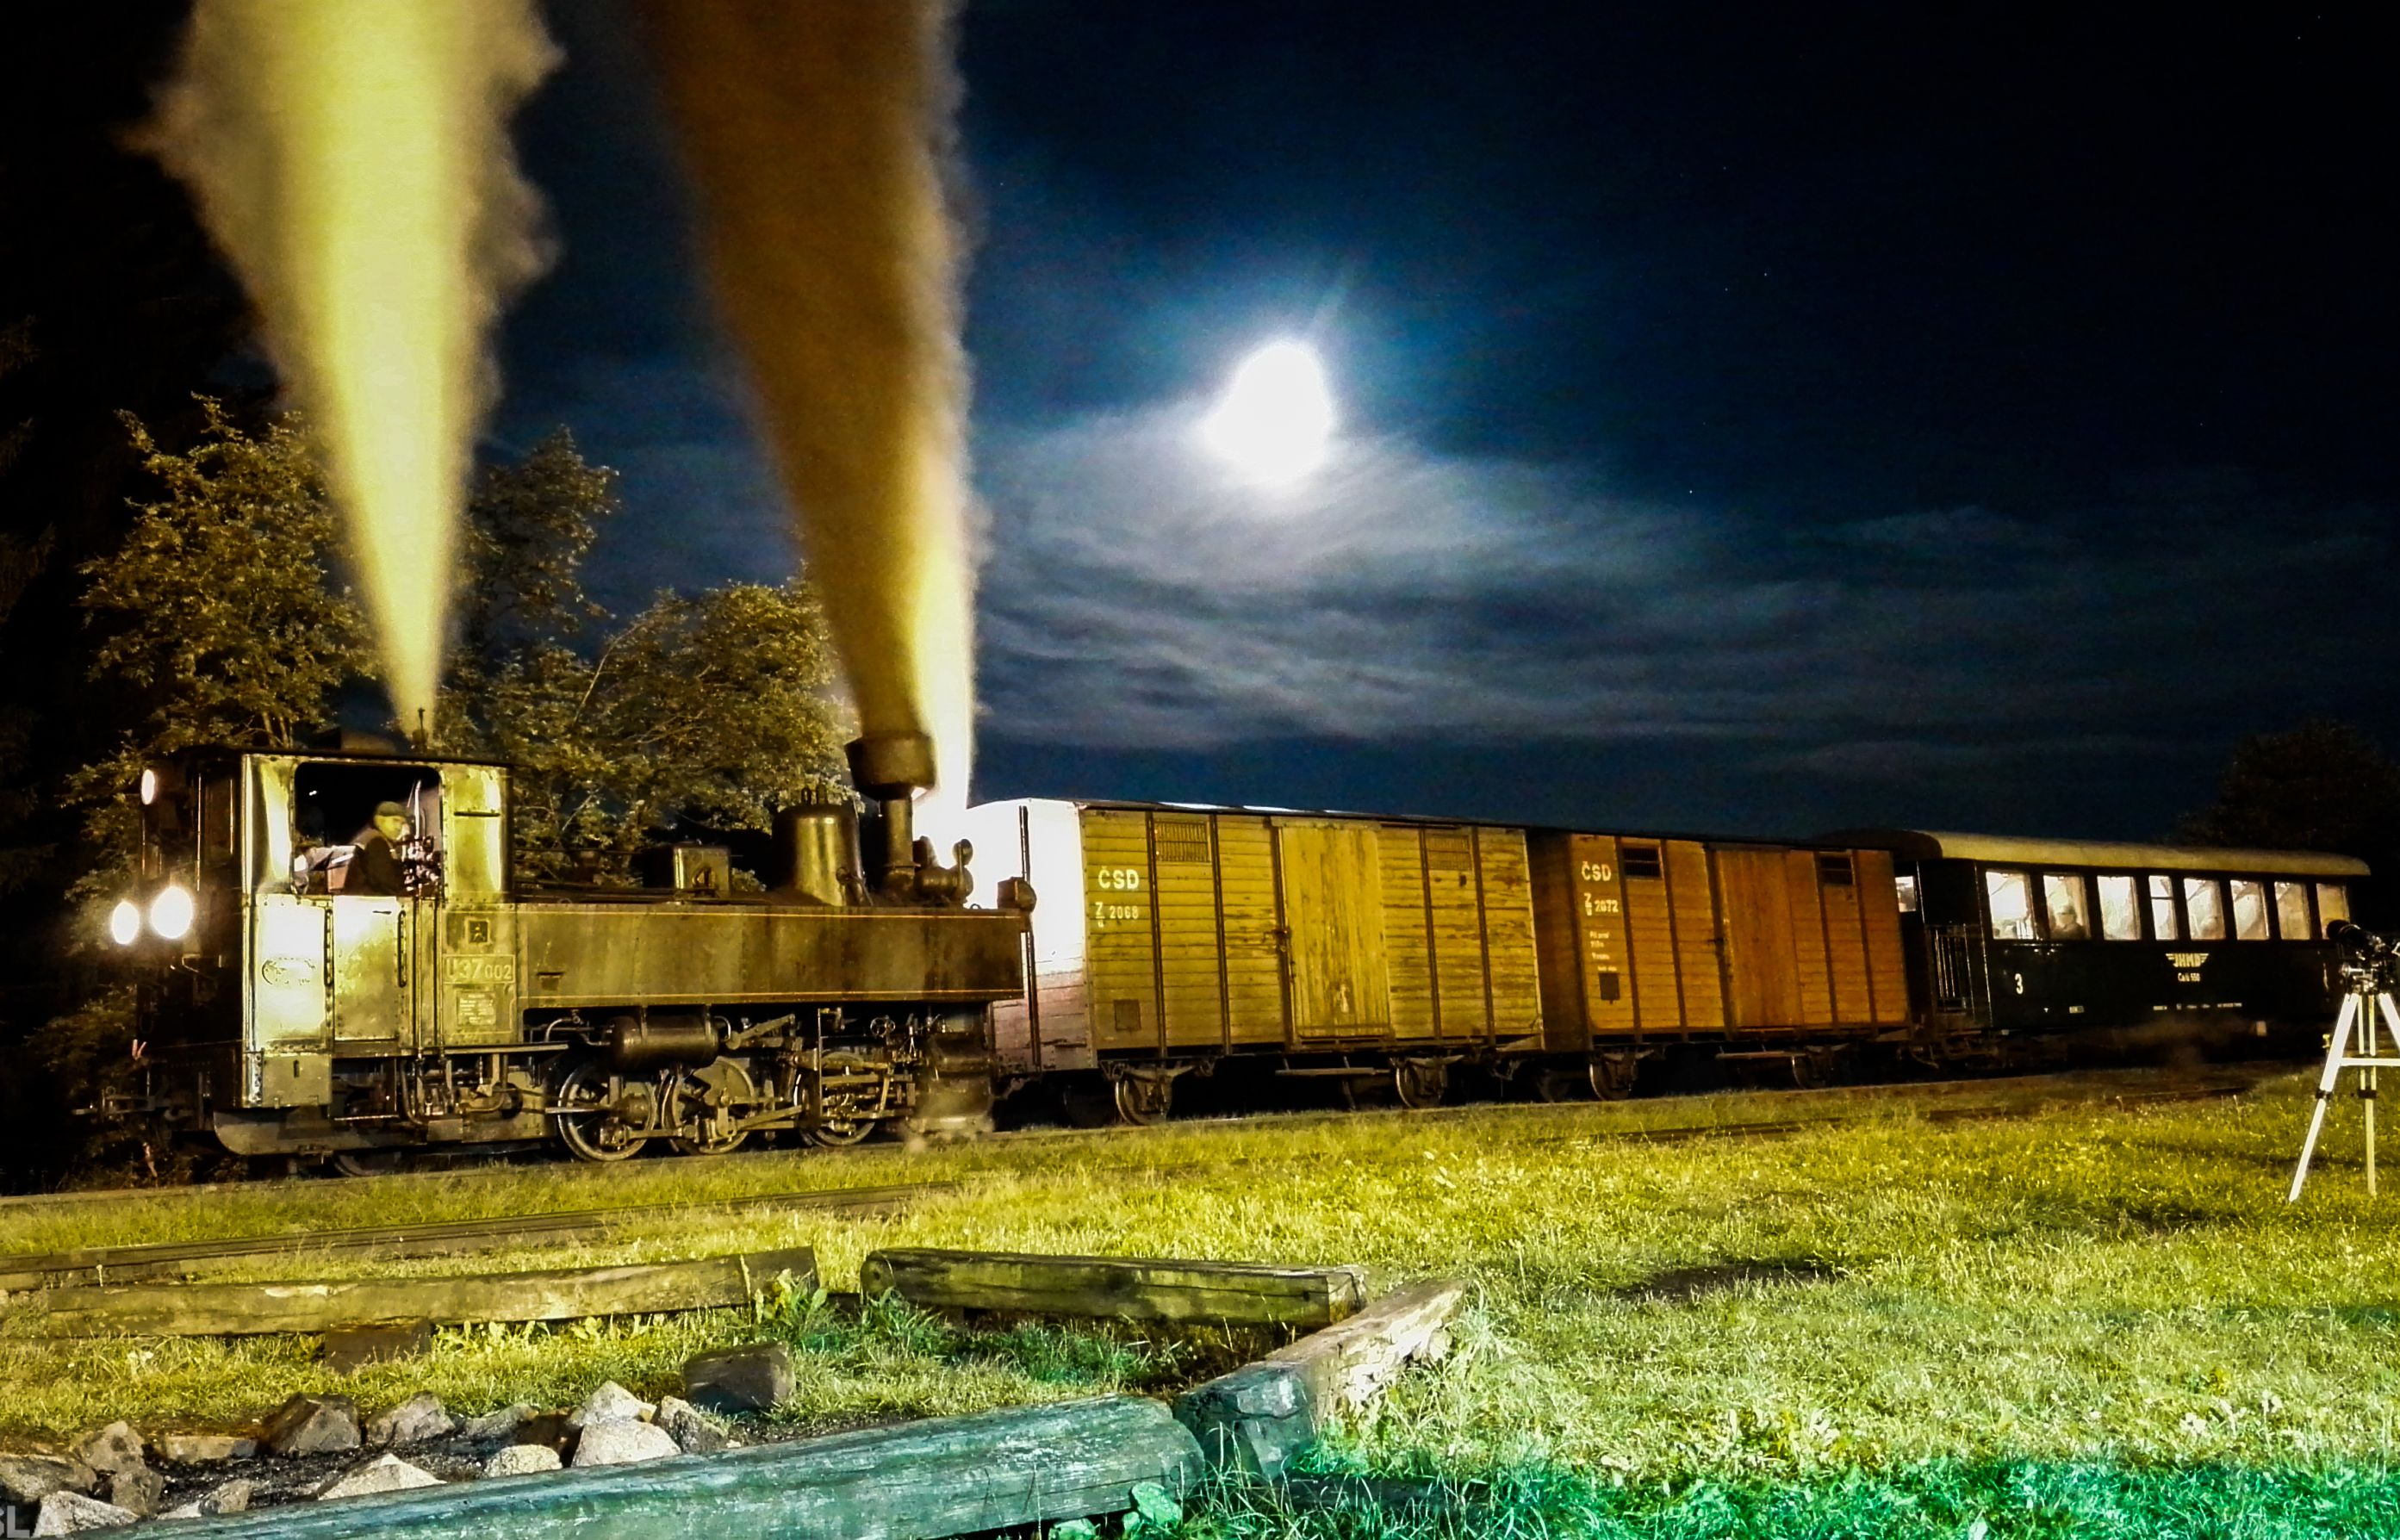
\includegraphics[width=\textwidth]{media/astrovlak/st.jpg}
\caption{Noční jízda vlaku}
\end{figure}
\vfill
\begin{figure}[ht!]
\centering
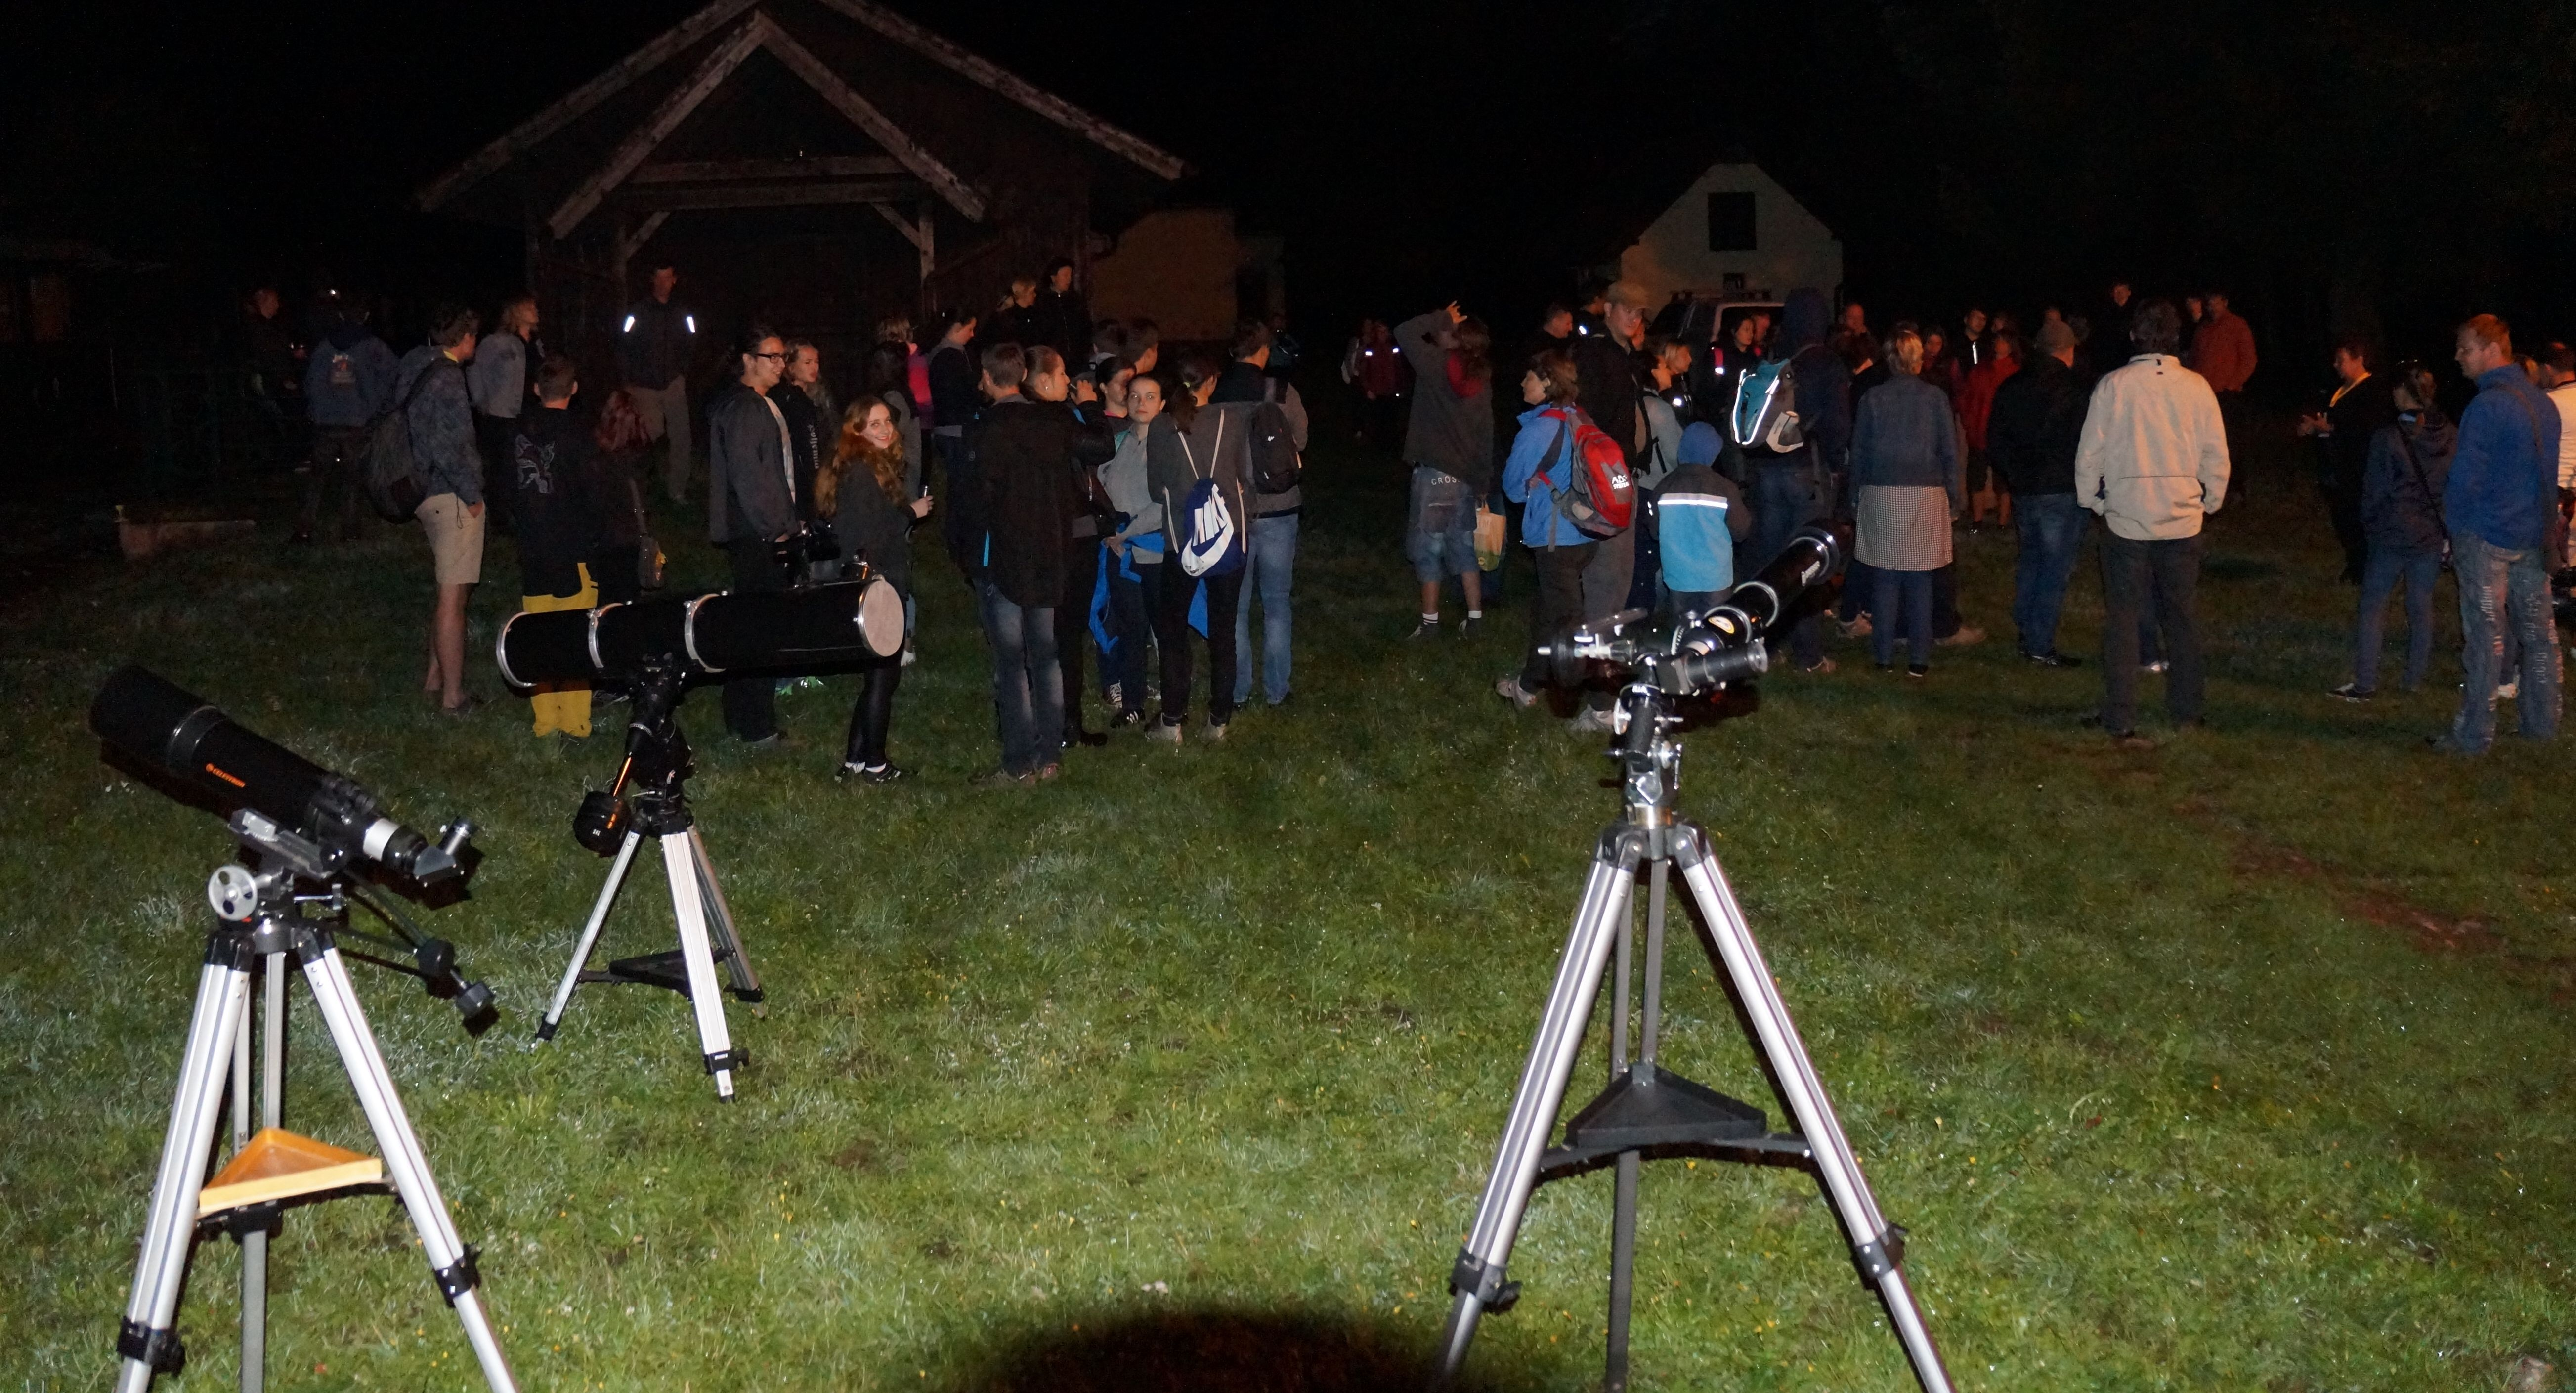
\includegraphics[width=\textwidth]{media/astrovlak/pozorovani.jpg}
\caption{Veřejné pozorování}
\end{figure}
\newpage
\nadpis{Ohlédnutí za 20. Sjezdem České astronomické společnosti}{Evžen Thöndel \\ člen Jihočeské pobočky, host na sjezdu.}

Vážení kolegové,
zúčastnil jsem se jako host za Jihočeskou pobočku České astronomické společnosti jejího 20. sjezdu. Delegáty za naši pobočku byli pánové Josef Szylar a Vladan Špaček. Byl jsem rád, že se mohu této akce zúčastnit a dost jsem byl překvapený, když jsem zjistil, že o účast není ani tak velký zájem. Vysvětlení je asi v hodnocení předešlých sjezdů. Tento sjezd však měl všechna „nej“. Rozepisovat se v této věci ani tak moc nechci. O hodnocení sjezdu jste se jistě dočetli v článcích na www.astro.cz. Proč jsem chtěl na sjezd vlastně jet. Jednoznačně proto, že jsem členem ČAS čtyři roky a chtěl jsem poznat i strukturu této společnosti. Chtěl jsem také využít tuto příležitost k volné diskuzi k některým odborným tématům, která se v naší pobočce řeší a poznat, jak jsou tato témata vnímána v celé ČAS. Z mého pohledu je to téma shrnuté v projektu „Bolidozor“ případně i navazující určité formě radioastronomie. Projekt nadmíru zajímavý.


Ale. Již na poslední členské schůzi Jihočeské pobočky ČAS jsem pociťoval jistou “váhavost“ nad tím, jak dále. Musí přiznat, že mě to znepokojilo.


Přivítal jsem proto možnost si na sjezdu o problému pohovořit s kolegy Josefem Szylarem a Vladanem Špačkem. Oba kolegové projevili zcela přesvědčivý zájem o projekt. Kolega Szylar navíc mohl podat i informace ze zrodu projektu a charakterizovat i některé současné těžkosti.



Osobně jsem chtěl také zjistit, jakou má náš projekt odezvu v profesionální části české astronomické společnosti. Dovolil jsem si proto využít téměř tříhodinovou společnou cestu vlakem s čestným předsedou, panem Dr. Jiřím Grygarem a naznačit náš problém. Chtěl jsem navázat na jeden z bodů usnesení sjezdu , a to je důraz na prohlubování spolupráce mezi profesionální a amatérskou částí naší společnosti. Výsledek, odezva v profesionální části ČAS, dle mého osobního názoru, je nevýrazná.
Současný stav našeho projektu „něco“ potřebuje. To je definovat cestu k cíli. To, co potřebuje, by mohlo být téma pro pracovní schůzku. O možném termínu a místu této schůze se domluvíme na výroční schůzi JihoČASu 25.11. na hvězdárně v Jindřichově Hradci.



\nadpis{Jak bylo na stoletém sjezdu}{Vladan Špaček, člen 3330}
Jak to vnímá amatér.


Velikou náhodou jsem byl delegován na sjezd České Astronomické Společnosti. Jako zájemce o astronomii , jenž se nazývá  "astronomem  amatérem" si uvědomuji svou "svatou"  povinnost ukazovat všem přátelům i náhodným kolem jdoucím vesmír v mém malém dalekohledu.  Jako člen ČAS jsem byl delegován do Brna na dvacátý sjezd u příležitosti  stého výročí této slovutné společnosti.


Už při příjezdu mne ohromila přesná a důkladná organizace. Vše se dělo velice samozřejmě, tak mne běh událostí jemně dotlačil do pohodlného křesla sjezdového sálu. Po začátku jednání a odhlasování úvodních formálních opatření pro průběh celé akce , po představení delegátů a kandidátů na nové vedení  společnosti následoval oběd. Úroveň cateringových služeb byla na mimořádně vysoké úrovni.


Organizátoři zajistili přejezd z planetária na koleje ,kde byli někteří delegáti ubytovaní. Zajistili formality s ubytováním a delegáty dovedli zpět na Kraví horu.


Po odpoledním programu následovalo nádherné vystoupení členů divadla Járy Cimrmana s  Dr. Zdeňkem  Svěrákem, prof. Miloňem Čepelkou, dr. Jiřím Grygarem, doc. Petrem Sobotkou a doc. Janem  Píšalou. Následně došlo k odhalením otisku boty Velikého Járy. Členové Jihočeské sekce ČAS prostřednictvím mé osoby předali  Panu Svěrákovi keramickou plastiku , ztvárňující černou díru vyrobenou z hlíny pořízené u Liptákova.


Následoval raut , který nikoho nenechal na pochybách, že se jedná o opravdu velkolepou akci. Při poslechu živé Jazzové hudby se konzumovali nejzrůznější dobroty, od lanýžů, zvěřiny  po roast beef. 


Další překvapení byl nádherný ohňostroj. \\ 
Na závěr sobotního večera pro nás organizátoři připravili fantastické promítání filmu o vzniku vesmíru .


Pak se šlo spát.\\
Dopoledne po bohaté snídani pokračovalo jednání sjezdu dle programu. Po zvolení nového vedení ČAS jsme se rozjeli domů.


Co dál říci.\\
Hostitelé sjezdu uspořádali akci , která si nezadá s akcemi na té nejvyšší úrovni. Sjezd byl velice významnou a důstojnou akcí, stejně jako je Česká astronomická společnost Slovutnou a důležitou organizací.





\nadpis{Zemřel Pavel Pavlovský}{Jana Jirků \\ Hvězdárna F. Nušla při DDM v Jindřichově Hradci}

Pan Pavel Pavlovský se narodil 6. prosince 1929 v Jindřichově Hradci. V šestatřicátém roce začal navštěvovat chlapeckou obecnou školu a o deset let později zahájil studium na střední škole průmyslové v Praze. Do prvního zaměstnání po absolvování vojny nastoupil do Rudného podniku v Praze a v roce 1958 se vrátil zpět do Jindřichova Hradce. Zde pracoval jako projektant na Okresním stavebním podniku celých 31 let.


\subsubsection*{První jindřichohradecký porevoluční místostarosta}
Pavel Pavlovský se postavil do čela vůbec prvního povolebního jednání zastupitelů v roce 1990. Protože byl nejstarším zvoleným kandidátem, vedl schůzi, ze které nakonec tajnou volbou vzešel jako první starosta Josef Eder. Za největší akci v době působení místostarosty Pavlovského na radnici považuje bývalý starosta prodej obecních bytů. „Městské byty na sídlištích se tehdy prodávaly do soukromého vlastnictví. Dělala se ale i řada jiných věcí, například se rekonstruovala kasárna u Hvězdárny, do provozu se také uváděla dnešní kolej VŠE a šestá základní škola,“ vzpomíná Petr Hudler.\\
(Zdroj: $http://jindrichohradecky.denik.cz/zpravy\_region/vzpominka-na- prvniho-mistostarostu-hradce-20170605.html$)

\subsubsection*{Hvězdárna a astronomie}
P. Pavlovský patřil k zakladatelům původního astronomického kroužku a měl nemalé zásluhy na rozvoji astronomie v regionu a na pozdějším vybudování Okresní lidové Hvězdárny v Jindřichově Hradci. V době krátkého výpadku činnosti hvězdárny, z důvodu tehdy plánovaného „jiného využití“ těchto prostor, byl cenným spojencem v našem boji o záchranu hvězdárny. Udržoval podrobný přehled o vývoji této neutěšené situace, poskytoval nám cenné informace, pomáhal ve všech krocích, jaké jsme jen mohli podniknout a dovedl zařídit i některé skutečnosti, jež bychom sami nikdy patrně neprosadili. Mezi ně např. patří to, že nám posvětil a oficiálně povolil vyjednat návštěvu Dr. Grygara na hvězdárně za účelem prohlídky a následného posouzení a vypracování odborné expertízy na světelné podmínky na hvězdárně.


Já osobně pamatuju pana Pavlovského jako milého, vstřícného a usměvavého člověka, který, pokud bylo třeba, vždy každému rád pomohl a vyhověl. Nikdy jsem ho nezažila rozčileného nebo se špatnou náladou, a to i v případě, když mu jednou v některém z autoservisů nekvalitně opravili auto ..... Veselá příhoda se odehrála cestou z hvězdárny, kdy mě p. Pavlovský svým autem vezl domů a vyprávěl mi o nekvalitě té opravy: zařadil rychlost, zakvedlal řadící pákou a celou ji vytáhl – prostě nedržela – se smíchem a slovy: "no tak se podívejte, kromě řazení mi to poslouží i jako klacek na sebeobranu!" Jen pro doplnění - z hvězdárny jsme jeli proto, že tehdejší dvojité dveře na pozorovací terasy, poničené vandaly, nešly po více než ročním výpadku zamykat a pan místostarosta Pavlovský sám koupil štítky a zámky a oboje dveře sám opravil!


Bohužel, p. Pavlovského velmi poznamenala smrt manželky, cca před dvěma roky. Od té doby často stonal a několikrát byl také hospitalizován v JH nemocnici. Začátkem prosince 2015 se ještě zúčastnil Předvánočního posezení na Hvězdárně F. Nušla, kde jsme mu slavnostně předali čestné členství na HFN a v Astroklubu. Zemřel ve středu 31. května 2017, ve věku nedožitých 88 let.
\begin{figure}[ht!]
\centering
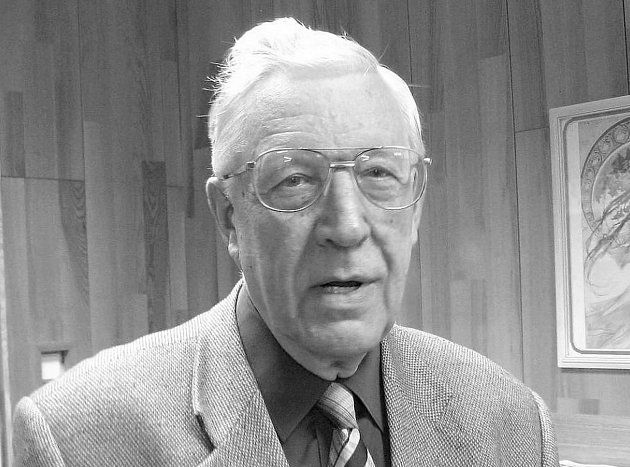
\includegraphics[width=0.9\textwidth]{media/pavel-pavlovsky.jpg}
\end{figure}
\begin{center}
\textbf{ČEST JEHO PAMÁTCE!}
\end{center}


\end{document}
 
 
%	\begin{itemize}
%	\item 
%	\end{itemize}
